
% this file is called up by thesis.tex
% content in this file will be fed into the main document

%: ----------------------- introduction file header -----------------------
%\begin{savequote}[50mm]
%Historical methodology, as I see it, is a product of common sense applied to circumstances.
%\qauthor{Samuel E. Morison}
%\end{savequote}


\chapter{Grupo de Schottky de la ecuaci\'on hipergeom\'etrica}
\label{cha:grupo schottky}

% the code below specifies where the figures are stored
%\ifpdf
  %  \graphicspath{{3_overall_methodology/figures/PNG/}{3_overall_methodology/figures/PDF/}{3_overall_methodology/figures/}}
%\else
 %   \graphicspath{{3_overall_methodology/figures/EPS/}{3_overall_methodology/figures/}}
%\fi


%-------------------------------------------------------------------------

%\cite{turing1950computing}

Nuevamente consideramos la ecuaci\'on hipergeom\'etrica

  $$x(1-x)\frac{d^{2}u}{dx^{2}} +  \lbrace c- (a+b+1 )x \rbrace \frac{du}{dx} - abu=0 $$

Cuyos exponentes son

$$ 1-c = i\theta_{0}, \ c-a-b = i \theta_{1},  \ a-b=i\theta_{2}  $$

Donde supondremos $\theta_{0}, \theta_{1} , \theta_{2} > 0$. Para cualesquiera dos soluciones linealmente independientes $u_{1}$ y $u_{2}$ tenemos el mapeo multivaluado $$s: \mathbb{C} -\lbrace0,1  \rbrace \ni x \mapsto u_{1}(x):u_{2}(x) \in \mathbb{P} := \mathbb{C} \cup \lbrace \infty \rbrace $$ llamado el mapeo de Schwarz.

\section{Dominios fundamentales}

 En \cite{geometricstudy} se pueden encontrar un  dominio $F_{x} $ en $\mathbb{C}$ y un dominio $F_{s}$ en $\widehat{\mathbb{C}}$ tal que el mapeo

 $$ s|_{F_{x}}: F_{x} \rightarrow F_{s}$$

  Es un biholomorfismo  y el mapeo $s$ se puede recuperar via el mapeo restringido $s|_{f_{x}}$ a traves del principio de reflexi\'on de Schwarz (\cite{geometricstudy}), estos se llaman dominios fundamentales para el mapeo de Schwarz. \\

\begin{figure}[h]
  \centering
  % Requires \usepackage{graphicx}
  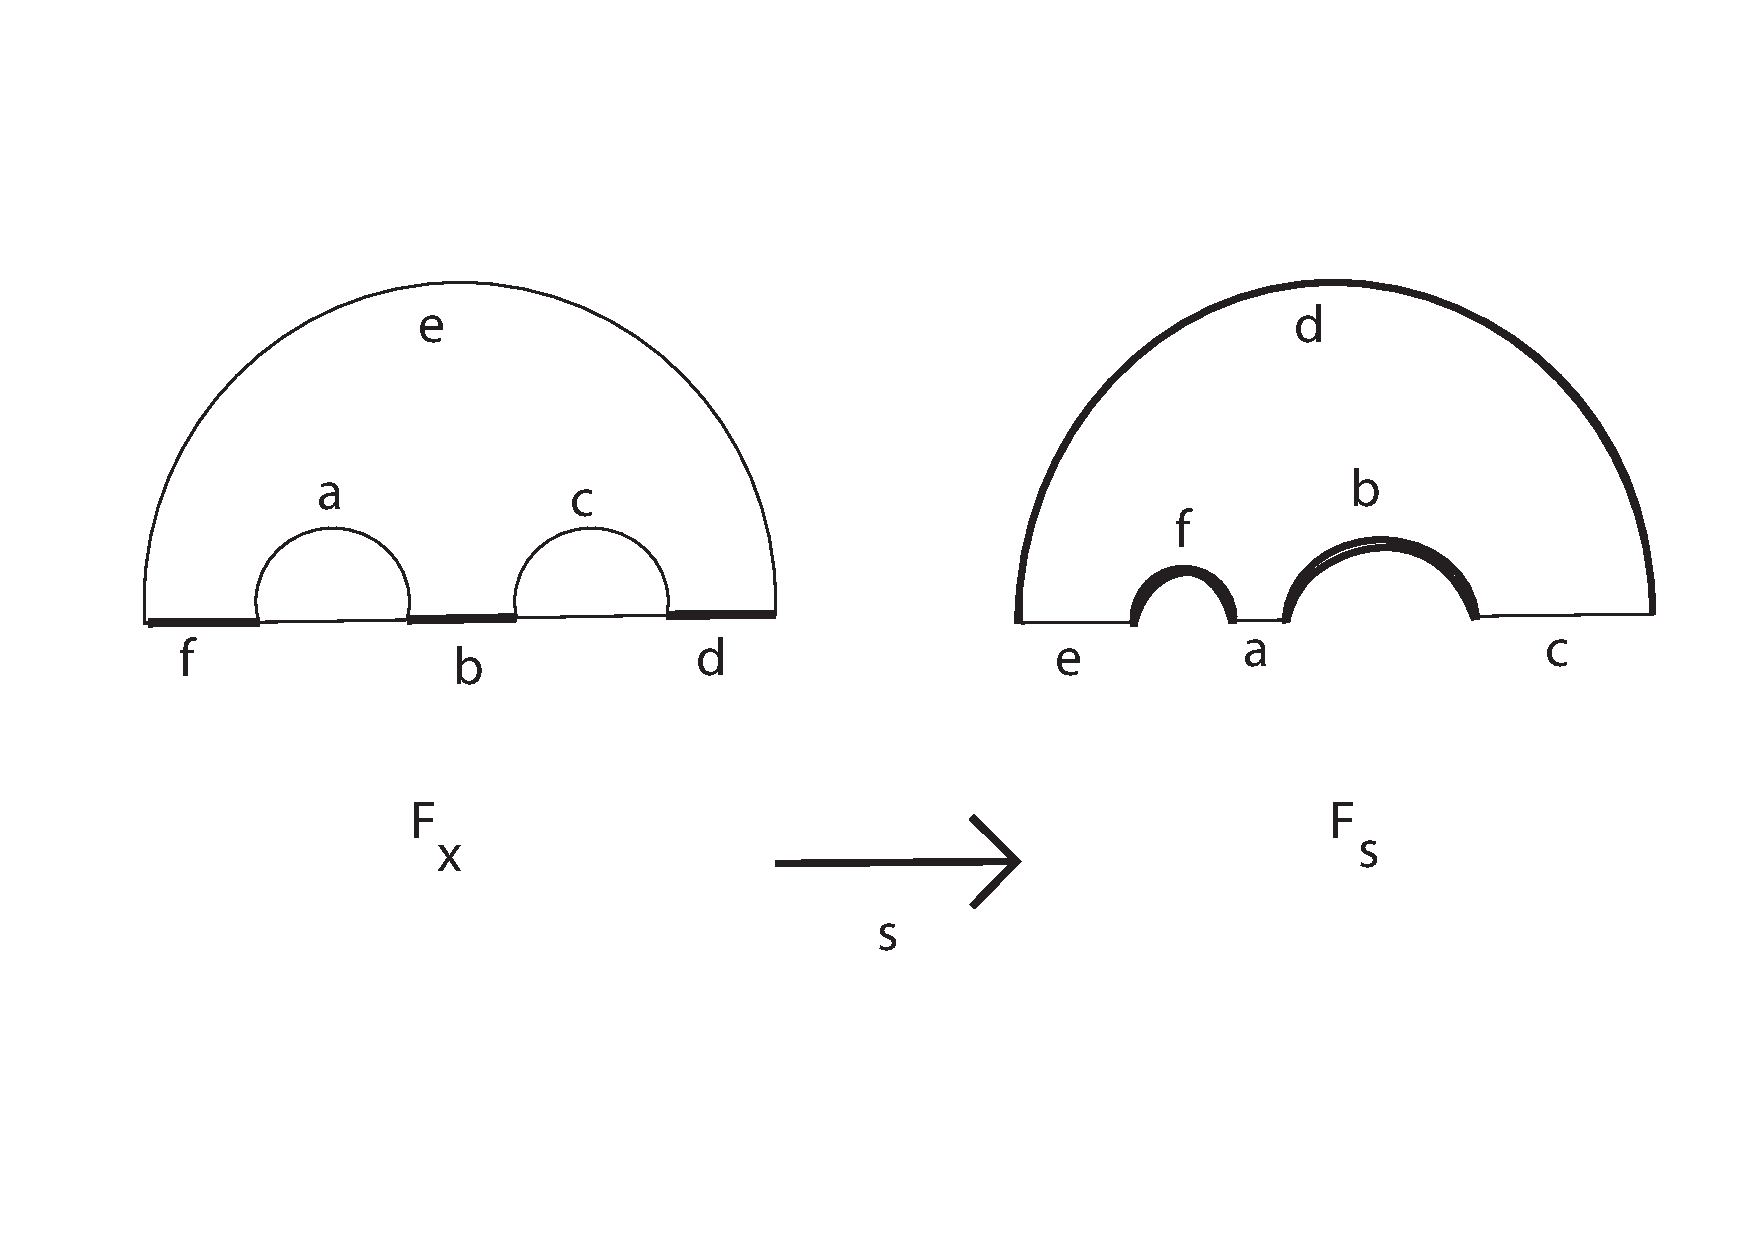
\includegraphics[width=10cm]{dominiosfundamentales.pdf}\\
  \caption{Dominios fundamentales}\label{dominiosfundamentales}
\end{figure}



Denotemos por $C(c,r)$ el c\'irculo en el plano $s$ con centro $c$ y radio $r$ y considerense los tres c\'irculos disjuntos en el plano $s$

$$ C_{1} = C(0,1), C_{2}=C(0,T), C_{3}= C(-C,R)$$

Donde $T=e^{\theta_{1} \pi}, r= e^{-\theta_{0} \pi}$

$$ C=\frac{\xi (1-r^{2})}{\xi^{2}-r^{2}},R=\frac{r(1-\xi^{2})}{\xi^{2}-r^{2}}, \xi =( \frac{cosh \theta_{2} \pi + cosh(\theta_{0}-\theta_{1}) \pi}{cosh \theta_{2} \pi + cosh(\theta_{0} + \theta_{1})\pi} )^{\frac{1}{2}}$$


Cuando $\theta_{2} = 0$

$$ Cosh (\theta_{0}-\theta_{1})\pi = \frac{1+(rt)^{2}}{2rT}$$

y

$$Cosh( \theta_{0} + \theta_{1})\pi = \frac{r^{2} + T^{2}}{2rT}$$

 Y tambi\'en $Cosh\theta_{2}\pi = 1 $ por lo que

 $$\xi^{2}|_{\theta_{2}=0} = \frac{1 + \frac{1 + (rt)^{2}}{2rT}}{ 1 + \frac{r^{2 } + T^{2}}{2rT}} = \frac{\frac{2rT + 1 + (rt)^{2}}{2rT}}{\frac{2rT + r^{2} + T^{2}}{2rT}}= \frac{T^{2} + 2rT +1}{r^{2} + 2rT + T^{2}} = \frac{(rT  + 1)^{2}}{(r + T)^{2}}$$

Entonces $\xi|_{\theta_{2}=0} = \frac{Tr + 1}{ T +r}$

Ya que $T>1$ y $r <1$ tenemos por un lado $r^{2}<1$ entonces $Tr + r^{2} < Tr + 1$, es decir, $r(T+r)< Tr +1$, entonces;$r<\frac{Tr + 1}{T+r}$.

Por otro lado; $r<1$ y tambi\'en $T-1>0$ por lo que $(T-1)r < T-1$ entonces $Tr-r < T-1$ y luego $Tr +1 < T+r$ por lo que $\frac{Tr +1}{T +r} < 1$
Dado que $\xi $ como una funci\'on de $\theta_{2} \geq 0$ incrementa de manera mon\'otona a 1 y $$1 > \xi |_{\theta_{2} =0} = \frac{Tr+1}{T+r} > r $$

tenemos

$$C-R-1 =\frac{\xi(1-r^{2})}{\xi^{2}-r^{2}} - \frac{r(1-\xi^{2})}{\xi^{2}-r^{2}}-1= \frac{\xi-\xi r^{2} -r + r\xi^{2}-\xi^{2} - r^{2}}{\xi^{2} - r^{2}}$$
$$= \frac{\xi-r + \xi r(-r + \xi)-(\xi -r)(\xi + r)}{ \xi^{2} - r^`{2}}$$
$$= \frac{(\xi -r)(1 + \xi r - (\xi +r))}{(\xi +r)(\xi -r)}$$
$$=\frac{1 + \xi r -(\xi +r)}{\xi +r}=\frac{(1-r)(1-\xi)}{\xi +r} > 0  $$

$$T-C-R =\frac{(T+r)\xi - (Tr +1)}{\xi -r} >0$$

y tenemos

$$-T < -C -R < -C + R < -1< 1< T $$

\begin{rem}
Existe una relaci\'on entre el n\'umero $\xi $ y los elementos de la matriz $P $ en el teorema \ref{matriz_conexion} y una relaci\'on entre dichos elementos, estas relaciones son importantes para verificar m\'as adelante que en efecto podemos decir que el grupo de monodrom\'ia de la ecuaci\'on hipergeom\'etrica es un grupo de $Schottky$, Las relaciones son las siguientes;

$$  \  P = \begin{pmatrix}
      D & C \\
      B & A
        \end{pmatrix} , \ \ \xi = \frac{|A|}{|B|}$$

 Y tambi\'en $A=\bar{D}, \ B= \bar{C}$
\end{rem}


El dominio en el semi-plano superior, acotado por $C_{1}, C_{2}, C_{3}$ y el eje real, puede servir como un dominio fundamental $F_{s}$, y tiene la forma de un puente de doble arco como en la figura \ref{dominiosfundamentales}. El dominio fundamental $F_{x}$ tambi\'en tiene la forma de de un  puente de doble arco como en la figura \ref{dominiosfundamentales}, y esta acotado por tres segmentos reales y tres curvas que no son parte de circunferencias.

\section{El grupo de monodrom\'ia generado por reflexiones}

Gracias a estos dominios fundamentales y el principio de reflexi\'on de Schwarz (\ref{cha:apendice}) aplicado a lo largo de los lados, el grupo de monodrom\'ia de la ecuacion diferencial se puede describir como sigue. La reflexi\'on con respecto al c\'irculo $C(c,r)$ donde $c$ es real, esta dada por  $$\psi(c,r): s \mapsto \frac{r^{2}}{\bar{s} - c}  $$

Sea $\bar{\Lambda}$ el grupo generado por las tres reflexiones respecto a los c\'irculos $C_{1},C_{2},C_{3}$, respectivamente. El grupo de monodrom\'ia $\Lambda_{\theta}$ de la ecuaci\'on hpergeom\'etrica es el subgrupo de $\bar{\Lambda}$, de \'indice 2 que consiste de las palabras pares de $\psi_{1},\psi_{2}, \psi_{3}$.

Por otro lado, para el c\'irculo $C(c,r)$ definimos la transformaci\'on fraccional lineal de orden 2 que fija los dos puntos de intersecci\'on del c\'irculo y el eje real: $$\gamma (c,r): s \mapsto \frac{r^{2}}{s-c} + c $$


Sea $\Gamma _{\theta},$ el grupo generado por tres involuciones $\gamma_{1},\gamma_{2},\gamma_{3}$ con respecto a los c\'irculos $C_{1},C_{2},C_{3}$, respectivamente.
El grupo de monodrom\'ia $\Lambda_{\theta }$ es el subgrupo de $\Gamma_{\theta}$, de \'indice 2 que consiste de las palabras pares de $\gamma_{1},\gamma_{2},\gamma_{3}$. Sea $\omega ( \subset \mathbb{P}^{1})$ el dominio de discontinuidad de $\Gamma_{\theta}$ y el grupo de Schotky $\Lambda_{\theta}$.

Esta representaci\'on tiene algunos problemas, aunque la ecuaci\'on hipergeom\'etrica es sim\'etrica respecto de $\theta_{0},\theta_{1},\theta_{2}$, los tres c\'irculos $C_{1},C_{2},C_{3}$ no lo son. Por ejemplo si $\theta_{2} \rightarrow 0$ los c\'irculos $C_{2}$ y $C_{3}$ se tocan, y si $\theta_{1} \rightarrow 0$ entonces $C_{3}$ tiende a un punto y $C_{1}$ y $C_{2}$ coinciden, m\'as a\'un ya que $C_{1}$  y $C_{2}$ son concentricos. Hacemos un cambio de coordenadas como sigue :

$$s \mapsto \frac{(3 + T^{2})s + 1 + 3T^{2}}{4(s + T^{2})} $$

 entonces los diametros de los c\'irculos en el eje real estan dados por

  $$ C_{1}:[s_{4},s_{5}],C_{2}:[s_{1},s_{6}],C_{3}:[s_{2},s_{3}]$$

\begin{figure}[h]
  \centering
  % Requires \usepackage{graphicx}
  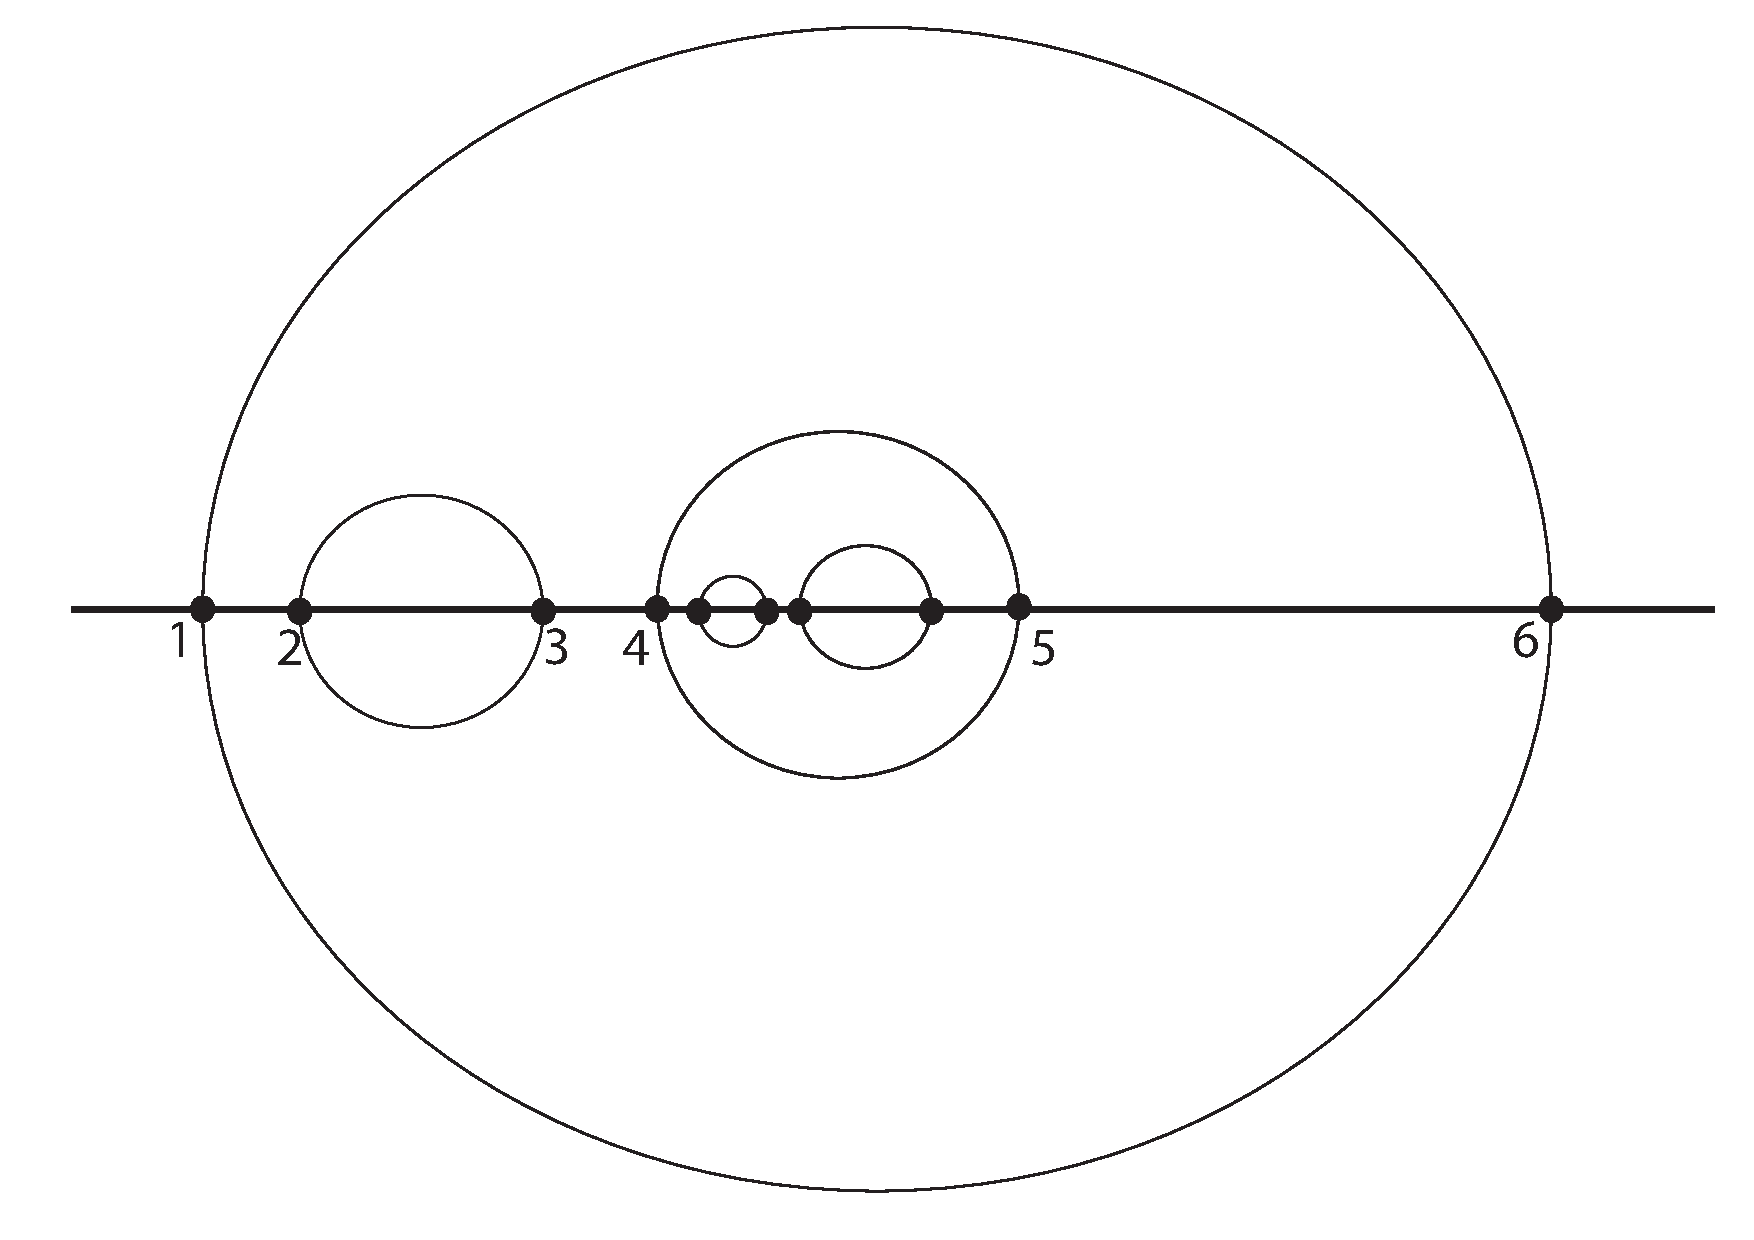
\includegraphics[width=10cm]{nuevosdiametros.pdf}\\
  \caption{C\'irculos $C_{1},C_{2},C_{3}$}\label{nuevosdiametros}
\end{figure}


Donde $$s_{1} = - \frac{(1-T)^{2}}{4T} , s_{2}= - \frac{(T-1)^{3} - (3 + T^{2})(T-C-R)}{4(T^{2} - T + T -C-R)}$$



$$s_{3}= -\frac{(1+T^{2})(C-R-1)}{4(T^{2}-1-(C-R-1))} + \frac{1}{2}, s_{4} = \frac{1}{2} $$

$$s_{5} = 1 , s_{6} = \frac{(1+ T)^{2}}{4T} $$


Notemos que $s_{1}< s_{2}< \cdots < s_{6}$, Ahora podemos probar lo siguiente,

\begin{prop} Si $\theta_{1} = 0$ entonces $C_{1}$  y $C_{2}$ se tocan en un punto. Si $\theta_{2} = 0 $ entonces $C_{2}$ y $C_{3}$ se tocan en un punto. Si $\theta_{0} = 0$, entonces $C_{3}$ y $C_{1}$ se tocan en un punto
\end{prop}

\textit{Prueba.}

Cuando $\theta_{1} = 0$, notemos que en este caso $T = e^{\theta_{1} \pi}$ y dado que $\theta_{1} = 0$ se tiene que $T =1$, tambi\'en recordemos que $C_{1}:[s_{4},s_{5}]$ y $C_{2}: [s_{1}, s_{6}]$ y dado que $s_{5} = 1 $ y $s_{6} = \frac{(1+ T^{2})^{2}}{4T} = \frac{(1 + 1^{2})^{2}}{4} = \frac{4}{4} = 1$ concluimos que $C_{1}$ y $C_{2}$ se tocan en $1$.

Si $\theta_{2} = 0$,primero veremos que $T-C-R = 0$, como $\theta_{2}=0$ entonces $\xi = \frac{Tr +1}{ T + r}$ esto implica que $(T+r) \xi = Tr +1$ y como $T-C-R = \frac{(T+r)\xi - (Tr+1)}{ \xi -r} = \frac{Tr+1 - ( Tr+1)}{\xi - r} =0$, Ahora bien $s_{1} = -\frac{1-T^{2}}{4T}$ y $s_{2} = -\frac{(T-1)^{3} - (3 + T^{2})(T-C-R)}{ 4(T^{2} - T + T-C-R)} =- \frac{(T-1)^{3}}{4(T^{2} - T)} =- \frac{(T-1)^{2} (T-1)}{4T (T-1)} = -\frac{(T-1)^{2}}{4T}= s_{1} $ por lo que $C_{2}$ y $C_{3}$ se tocan en $s_{1}$.

Por \'ultimo si $\theta_{0} = 0$ tenemos $r=e^{-\theta_{0} \pi }$ en este caso $r = 1$ mostremos que $C-R-1=0$.De las deducciones anteriores $C-R-1 = \frac{(1-r)(1- \xi)}{ \xi + r}$,Entonces $C-R-1= 0$ ya que $r = 1$, entonces $ s_{3} = \frac{(1+T^{2})(C-R-1)}{ 4(T^{2} -1 -C-R-1)} + \frac{1}{2} = \frac{1}{2}$ ya que $C-R-1 = 0$ y dado que $C_{3}:[s_{2},s_{3}]$ y  $ C_{1}:[s_{4},s_{5}]$ por los calculos anteriores obtuvimos $s_{4}= s_{3}$ (recordando que $s_{4} = \frac{1}{2}$), Concluyendo con la prueba. $\square $



\section{ El grupo de Schottky asociado al grupo de Monodrom\'ia}

Si ahora tomamos como antes las reflexiones $\psi_{1},\psi_{2},\psi_{3}$, definimos las siguientes transformaciones;

$$\gamma_{1}=\psi_{2} \psi_{1} \ , \ \gamma_{2} = \psi_{1} \psi_{3} $$

Y tomamos los c\'irculos $C_{1}, C_{3}$ y $C_{1}' = \psi_{2} (C_{1}), C_{3}'= \psi_{1} (C_{3})$, luego por definici\'on tenemos;

$$\gamma_{1} ( C_{1})= C_{1}'  \ \ , \ \ \gamma_{2} (C_{3}) = C_{3}'$$

Adem\'as tenemos que el exterior de $C_{1}$ se mapea al interior de $C_{1}'$ y el exterior de $C_{3}$ se mapea al interior de  $C_{3}'$, por la definici\'on tenemos un grupo de $Schottky$ de genus 2 (genero 2). Para el grupo de $Schottky$ anterior tenemos que sus transformaciones estan dadas tambi\'en por;

$$\gamma_{1}= sT^{2} \leftrightarrow   \begin{pmatrix}
 1& 0\\
 0& \frac{1}{T^{2}}
 \end{pmatrix} \  ,  \ \gamma_{2} = \frac{s + C}{ -Cs + R^{2} - C^{2}}  \leftrightarrow  \begin{pmatrix}
 1& C\\
 -C&  R^{2} - C^{2}
 \end{pmatrix}   $$

Y notando que $C=\frac{|A||B|(1-r^{2})}{|A|^{2}-|B|^{2}r^{2}}$ y $R^{2} - C^{2} =\frac{|A|^{2}r^{2}-|B|^{2}}{|A|^{2}-|B|^{2}r^{2}} $ podemos ver  que son conjugadas bajo $P$ a las matrices del grupo de monodrom\'ia de la ecuaci\'on hipergeom\'etrica \ref{Matrices_teorema_monodromia_grupo}.
% ----------------------------------------------------------------------

